\chapter{Lecteur de cartes}
Afin de vérifier l'assiduité des élèves lors des conférences nous mettons en
place un système de badge.

Il nous fallait une solution alliant plusieurs critères comme un coût et temps
de développement réduit et de la fabilité.

\newpage

\section{Historique}
Dès le début du projet Monsieur Berry nous a proposé plusieurs pistes à 
explorer pour le badge en lui même. Il fallait que chaque participant aux
conférences puisse être identifié de manière unique:

\begin{itemize}
\item Money Kart: C'est une entreprise basée près de Grenoble, spécialisée
dans la création de cartes à puce, notamment Moneo. L'avantage de cette solution
résidait dans la design des cartes. On aurait pu les faire graver
de façon à faire un buzz autour de la Semaine du Numérique. De plus la société
vendait également des lecteurs prêts à l'emploi.
Malheuresement, il nous fût impossible d'obtenir un devis de la part d'un
commercial, même après de multiples relance. Cette solution nécéssitait aussi
un investissement financier.

\item Carte étudiantes: Rapidement cette solution à fait l'unanimité. En effet,
elle était bien plus facile à mettre en place: chaque titulaire de carte délivrée
par l'UM2 possède un numéro unique, appelé numéro Mifare, accessible grâce à
la technologie RFID. Or Polytech possède une base de donnée faisant le lien entre
ce numéro et les élèves.
\end{itemize}

\section{RFID et Mifare}
RFID, de l'anglais ``radio frequency identification'' est une techonlogie 
mise au point pour permettre de lire à distance des données contenues dans des
marqueurs, étiquettes RFID.

    \begin{figure}[h]
        \begin{center}
            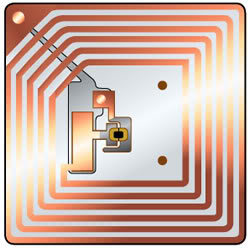
\includegraphics[scale=0.6]{RFIDtag.jpg} 
        \end{center}

        \caption{Etiquette RFID}
        \label{Etiquette RFID}
    \end{figure}


C'est une technologie employée quotidiennement par tout le monde puisqu'elle
sert entre autre à:

\begin{itemize}
\item Passeport bimométrique français.
\item Accès transport public, comme le tramway de Montpellier.
\item Inventaires.
\end{itemize}

Mifare est une des technologies de carte à puce sans contact les plus répandues
dans le monde avec 3,5 milliards de cartes et 40 millions de modules de lecture/encodage.

Ces deux technologies respectent des normes ISO.

\section{Cahier des charges}
%demander a catebras et tanby si les citer ne les dérange pas
Avant tout, la décision de mise en place d'un lecteur de carte correspond au désire d'un gain 
de temps et de facilité d'utilisation. De plus cela revêt un côté écologique dans le sens 
où la consommation de papier ne sera pas afféctée par les fiches d'appels. Mr G.Catebras en 
collaboration avec Mr J.Tanby et V.Berry ont décidé de mettre en place le lecteur pour palier aux
 défauts du lecteur (MFR120U).\newline
\subsection{problème posé}
Le module MFR120U remplissait sa fonction principal mais doit être substitué à cause des défauts suivant:
\begin{itemize}
\item pour avertir qu'une carte a bien été badgée, le module doit pouvoir générer un signal lumineux clairement visible. Le MFR120U possède une led mais elle est cachée car la carte de l'étudiant lors du badgage. Un signal sonore étant à bannir dans les salle de cours ou même dans un amphithéatre.
\item sa taille trop petite et sa forme.
\end{itemize}
De ce fait nous avons mis en place un programme de badgage dont le fonctionnement est analoque à celui du MFR120U qui sera utilisé de concert avec le module fournit par Mr J.Tanby que nous avons rencontré pour lui notifier les caractéristiques voulues ainsi que la technologie qu'il devait utiliser pour communiquer en bluethoot, pour que le programme (nous avon commensé le codage de l'application en nous basant sur le MFR120U) soit compatible avec le module qu'il créera et pour minimiser au maximum les modifications à aporter. \newline
%TODO: parler du protocole
\subsection{Expression fonctionnelle du besoin}
Les principales fonctions du programmes sont:
\begin{itemize}
\item 
\end{itemize}
\subsection{Les solutions proposées pour répondre à ce besoin}
\begin{itemize}
\item 
\end{itemize}
\section{Modélisation}
\section{Recommandations}
